\documentclass[xcolor=dvipsnames]{beamer}

\mode<presentation>
% these codes for chinese characters input, if you meet problems with these codes, you can feel free to comment them, or you can try to change your build method to "xelatex"
% \documentclass[xcolor=dvipsnames]{beamer}
% \usepackage{xeCJK}
\usepackage{verbatim}
\usepackage{subfigure} 
\RequirePackage{color}
% For convenience, some of the topics are listed here for users to use.

% \usetheme{AnnArbor}
%\usetheme{Antibes}
%\usetheme{Bergen}
% \usetheme{Berkeley}
%\usetheme{Berlin}
%\usetheme{Boadilla}
% \usetheme{boxes}
% \usetheme{CambridgeUS}
%\usetheme{Copenhagen}
%\usetheme{Darmstadt}
% \usetheme{default}
%\usetheme{Frankfurt}
%\usetheme{Goettingen}
%\usetheme{Hannover}
% \usetheme{Ilmenau}
% \usetheme{JuanLesPins}
%  \usetheme{Luebeck}
 \usetheme{Madrid}
% \usetheme{Malmoe}
%\usetheme{Marburg}
% \usetheme{Montpellier}
% \usetheme{PaloAlto}
% \usetheme{Pittsburgh}
% \usetheme{Rochester}
% \usetheme{Singapore}
% \usetheme{Szeged}
% \usetheme{Warsaw}

\definecolor{sjtu-red}{RGB}{184,45,40} 
\definecolor{sjtu-white}{RGB}{255,255,255}
\definecolor{sjtu-blue}{RGB}{21,65,146}
\definecolor{sjtu-black}{RGB}{0,0,0}

% Uncomment the following code to get the color gradient on the slide (Decaying from sjtu-red to sjtu-white).


% \useoutertheme{shadow}
% \usepackage{tikz}
% \usetikzlibrary{shadings}
% \colorlet{titleleft}{sjtu-red}
% \colorlet{titleright}{sjtu-red!45!sjtu-white}
% \makeatletter
% \pgfdeclarehorizontalshading[titleleft,titleright]{beamer@frametitleshade}{\paperheight}{%
%   color(0pt)=(titleleft);
%   color(\paperwidth)=(titleright)}
% \makeatother

% End of gradient slide title effect.

\setbeamercolor{section in head/foot}{bg=sjtu-blue, fg=sjtu-white}
\setbeamercolor{subsection in head/foot}{bg=sjtu-blue, fg=sjtu-white}
\setbeamercolor{frametitle}{bg=sjtu-blue, fg=sjtu-white}
\setbeamercolor{title}{bg=sjtu-blue, fg=sjtu-white}
\setbeamercolor{alerted text}{fg=sjtu-blue}
\setbeamercolor{block title}{fg=sjtu-white}
\setbeamercolor{block body}{fg=sjtu-black}

\setbeamertemplate{theorems}[numbered]
\setbeamertemplate{propositions}[numbered]

\setbeamertemplate{bibliography item}{\insertbiblabel}

\setbeamertemplate{title page}[default][colsep=-4bp,rounded=true, shadow=true]

\title[PI Measure]{PI Measure: A Set-Theoretic View of Partial Information}

\subtitle{2020 Spring CS258 Group Project Presentation}

% You can uncommit one of this code block to change
% from one-author's mode to muli-author's mode which is 
% displayed in the title page.
% \author{Authors' name}
% \institute[Shanghai Jiao Tong University] % (optional, but mostly needed)
% {
%   School of Electronic Information and Electrical Engineering\\
%   Shanghai Jiao Tong University
% }

\author[L. Zhou, H. Yang, S. Dong] {Litao Zhou, Hongbo Yang, Shiwen Dong}

\institute[SJTU-IEEE] % (optional)
{
  IEEE Class F1803016 \\
  School of Electronic Information and Electrical Engineering\\
  Shanghai Jiao Tong University
}

\titlegraphic{
  % Uncomment the other code line below to change the logo from English version to Chinese.  
   % 
\includegraphics[width=4.4cm]{sjtu-logo}
   
\includegraphics[width=4cm]{img/sjtu-logo-en.png}
}

\date{\today}

% Uncomment this, if you want the table of contents to pop up at the beginning of each subsection:

% End of the table-content part
% \AtBeginSection[]
% {
%   \begin{frame}{Outline}
%       \tableofcontents[currentsection,currentsubsection,hideothersubsections]
%   \end{frame}
% }
\begin{document}

\begin{frame}
  \titlepage
\end{frame}

\logo{
\includegraphics[height=1cm]{img/sjtu.png}}

% \begin{frame}{Outline}
%   \tableofcontents[hideallsubsections]
% \end{frame}


\section{Background}

\begin{frame}{Background}% {Optional Subtitle}
\begin{block}{I-Measure}
  A theory which establishes a one-to-one correspondence between Shannon's information measure and set theory in full generality.

    \begin{equation}\begin{aligned}
    H / I & \leftrightarrow \mu^{*} &&  , & \leftrightarrow \cup \\
    ; & \leftrightarrow \cap &&    | & \leftrightarrow -
    \end{aligned}\end{equation}
\end{block}

\begin{block}{Non-negative Decomposition of Multivariate Information}
  A measure of \emph{redundancy information} that a set of sources provides about a given variable.
  
  Shannon information can be decomposed into atoms of non-negative \emph{partial information}.
\end{block}


Our Goal: Using the I-Measure methodology to study the redundancy measure, forming a set-theoretic view of partial information.

\end{frame}



\section{I-Measure}


\subsection{Definition}
\begin{frame}{Definition}
    \begin{definition}[Field]
        The field $\mathcal{F}_{n}$ generated by sets $\tilde{X}_{1}, \tilde{X}_{2}, \cdots, \tilde{X}_{n}$ is the collection of sets which can be obtained by any sequence of usual set operations (union, intersection, complement, and difference) on $\tilde{X}_{1}, \tilde{X}_{2}, \cdots, \tilde{X}_{n}$
    \end{definition}
    
    
    \begin{definition}[Atom]\label{atom}
    The atoms of $\mathcal{F}_{n}$ are sets of the form $\cap_{i=1}^{n} Y_{i},$ where $Y_{i}$ is either$\tilde{X}_{i}$ or $\tilde{X}_{i}^{c},$ the complement of $\tilde{X}_{i}$\\
    \end{definition}
    
    
    \begin{definition}[Signed Measure]\label{sm}
    A real function $\mu$ defined on $\mathcal{F}_{n}$ is called a signed measure if it is set-additive, i.e., for disjoint $A$ and $B$ in $\mathcal{F}_{n}$
    \begin{equation}
    \mu(A \cup B)=\mu(A)+\mu(B)
    \end{equation}
    \end{definition}

\end{frame}


\subsection{Measure Theorem}
\begin{frame}{Measure Theorem}
    
    Use $X_{G}$ to denote $\left(X_{i}, i \in G\right)$ and $\tilde{X}_{G}$ to denote $\cup_{i \in G} \tilde{X}_{i}$ for any nonempty subset $G$ of $\mathcal{N}_{n} =\{1,2, \cdots, n\}$\\
 

    \begin{theorem}[Completeness]\label{th1}
    Let
    \begin{equation}
        \mathcal{B}=\left\{\tilde{X}_{G}: G \text { is a nonempty subset of } \mathcal{N}_{n}\right\}
    \end{equation}
    Then a signed measure $\mu$ on $\mathcal{F}_{n}$ is completely specified by $\{\mu(B), B \in \mathcal{B}\}$
    which can be any set of real numbers.
    \end{theorem}
    
    With the terminologies of measure theory above, we can construct a correspondence between set theory and Shannon Information
    
    
\end{frame}

\subsection{Correspondence}

\begin{frame}{Correspondence}
    \begin{block}{Build Correspondence}
    We now construct the I-Measure $\mu^{*}$ on $\mathcal{F}_{n}$ using Theorem \ref{th1} by defining%%%%%%%%%%%%%
    \begin{equation}
        \mu^{*}\left(\tilde{X}_{G}\right)=H\left(X_{G}\right)
    \end{equation}
    for all nonempty subsets $G$ of $\mathcal{N}_{n} .$ 
    
    The following must hold for all (not necessarily disjoint) subsets $G, G^{\prime}, G^{\prime \prime}$ of $\mathcal{N}_{n}$:
    \begin{equation}\label{eqx1}
        \mu^{*}\left(\tilde{X}_{G} \cap \tilde{X}_{G^{\prime}}-\tilde{X}_{G^{\prime \prime}}\right)=I\left(X_{G} ; X_{G^{\prime}} | X_{G^{\prime \prime}}\right)
    \end{equation}
    \end{block}
\end{frame}


\subsection{Applications}
\begin{frame}{Applications}
    \begin{block}{Information Diagrams}
        With the correspondence above, it is reasonable to use an \emph{information diagram}, which is a variation of Venn diagram, to represent the relationship between Shannon's information measures.
    \end{block}
    \begin{figure}
        \centering
        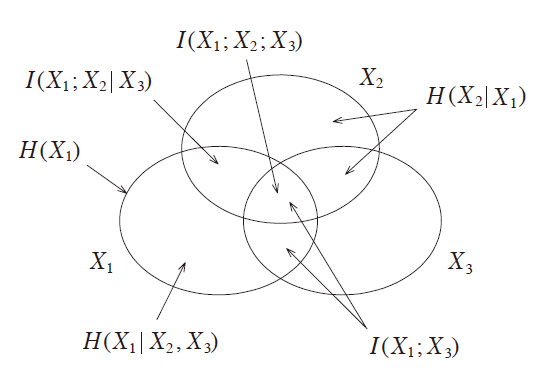
\includegraphics[height = 3cm]{img/Im3.png}
        \caption{Generic Information Diagram for $X_1, X_2, X_3$}
        \label{fig:genericID}
    \end{figure}
\end{frame}

\begin{frame}{Applications}
    \begin{block}{Information Diagrams for Zero Measure}
        In Markov Chain $X_{1} \rightarrow X_{2} \rightarrow X_{3}$, since \begin{equation}\mu^{*}\left(\tilde{X}_{1} \cap \tilde{X}_{2}^{c} \cap \tilde{X}_{3}\right)=I\left(X_{1} ; X_{3} | X_{2}\right)=0\end{equation}
        We don't have to plot that region out in the information diagram, making the diagram simpler and more useful when reasoning about Shannon information measures.
    \end{block}
    \begin{figure}
        \centering
        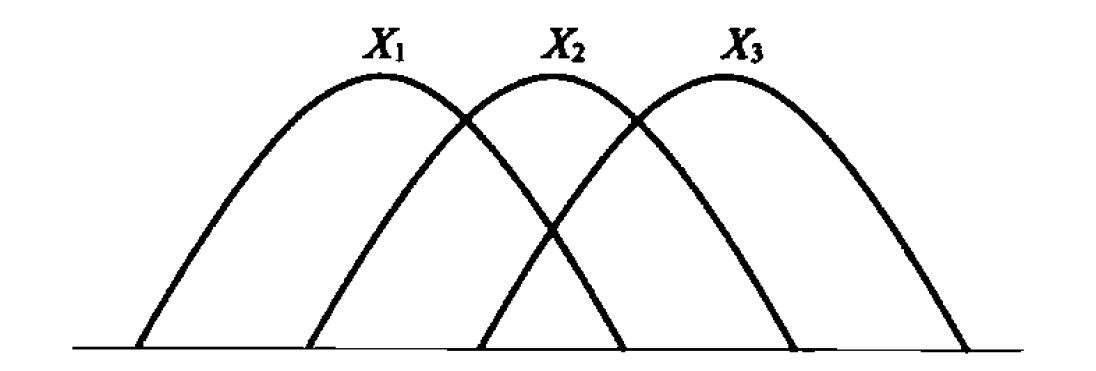
\includegraphics[height = 2cm]{img/Im4.png}
        \label{fig:MCID}
    \end{figure}
    
    In a word, with the set-theoretic view of information diagram, we can discover many useful properties.
\end{frame}


\section{Partial Information}
\subsection{Redundancy Measure}
\begin{frame}{Redundancy Measure}
    Let $A_1, A_2, \ldots, A_k$ be nonempty and potentially overlapping
subsets of $R,$ which we call sources. We introduce $I_{\min}$ to measure the information that all sources provide about S.
\begin{definition}[Redundancy Measure]
\begin{equation}I_{\min }\left(S ;\left\{\mathbf{A}_{1}, \mathbf{A}_{2}, \ldots, \mathbf{A}_{k}\right\}\right)=\sum_{s} p(s) \min _{\mathbf{A}_{i}} I\left(S=s ; \mathbf{A}_{i}\right)\end{equation}
where the domain of $I_{\min}$ $\mathcal{A}(\mathbf{R})=\left\{\alpha \in \mathcal{P}_{1}\left(\mathcal{P}_{1}(\mathbf{R})\right): \forall \mathbf{A}_{i}, \mathbf{A}_{j} \in \alpha, \mathbf{A}_{i} \notin \mathbf{A}_{j}\right\}$
\end{definition}

\begin{block}{Properties of Redundancy Measure}
\begin{itemize}
    \item $I_{\min}$ is non-negative
    \item $I_{\min }$ is less than or equal to $I\left(S ; \mathbf{A}_{i}\right)$ for all $\mathbf{A}_{i}$ 's
    \item For a given source A, the amount of information redundant with $\mathbf{A}$ is maximal for $I_{\min }(S ;\{\mathbf{A}\})=I(S ; \mathbf{A}) .$
\end{itemize}
\end{block}
\end{frame}

\subsection{Relations between Redundancy Measures}
\begin{frame}{Relations between Redundancy Measures}
    Note that $I_{\min}$ can measure redundancy between collections of sources like $\left\{\left\{R_{1}\right\},\left\{R_{2}, R_{3}\right\}\right\}$ denoted as $\{1\}\{23\}$. Certain relations exists between measures.
    
    \begin{columns}
    \begin{column}{0.5\linewidth}
        \centering
        \begin{block}{Redundancy Order}
            We can define a partial order over the elements of $A(R)$ such that one is considered to precede another if and only if the latter provides any redundant information that the former provides. Formally,
            \begin{equation}\begin{aligned}&\forall \alpha, \beta \in \mathcal{A}(\mathbf{R}), \\
            &\alpha \preccurlyeq \beta \Leftrightarrow \forall \mathbf{B} \in \beta, \exists \mathbf{A} \in \alpha, \mathbf{A} \subseteq \mathbf{B}\end{aligned}\end{equation}
        \end{block}
    \end{column}
    \begin{column}{0.45\linewidth}
        \begin{figure}
            \centering
            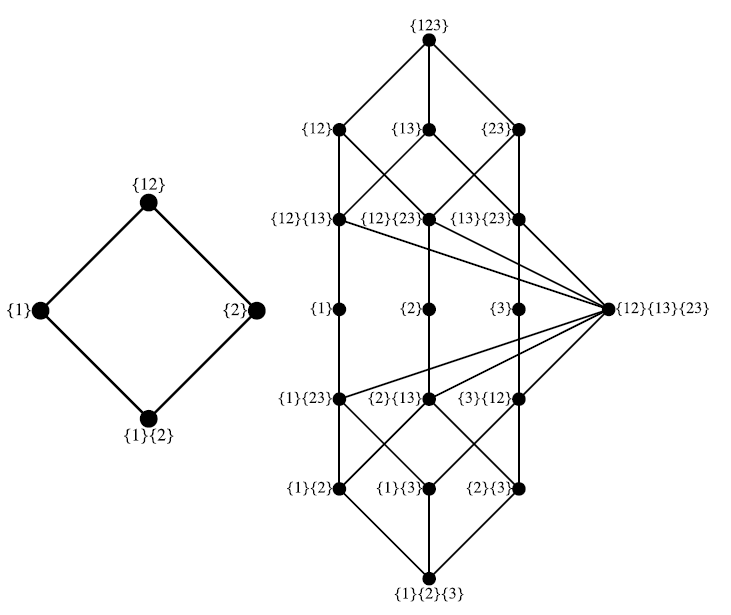
\includegraphics[width=0.8\linewidth]{img/lattic.png}
            \caption{Redundancy lattice for (A) 3 and (B) 4 variables.}
            \label{fig:lattice}
        \end{figure}
    \end{column}
    \end{columns}
\end{frame}

\subsection{Partial Information Decomposition}
\begin{frame}{Partial Information Decomposition}
    We would like to decompose redundancy measure into non-intersecting fragments. For a collection of sources $\alpha \in \mathcal{A}(\mathbf{R}),$ the PI-function denoted $\Pi_{\mathrm{R}},$ is defined implicitly by
    \begin{equation}
    I_{\min }(S ; \alpha)=\sum_{\beta \preccurlyeq \alpha} \Pi_{\mathrm{R}}(S ; \beta)
    \label{eee}
    \end{equation}
    
    \begin{columns}
    \begin{column}{0.5\linewidth}
    \begin{block}{Properties of Redundancy Measure}
    \begin{itemize}
        \item $\mathrm{II}_{\mathrm{R}}$ is non-negative
        \item $\mathrm{II}_{\mathrm{R}}$ can be calculated recursively.
        \item The relationship between these measures can be shown in a partial information (PI) diagram, which we will discuss later.
    \end{itemize}
    \end{block}
    \end{column}
    \begin{column}{0.45\linewidth}
        \begin{figure}
            \centering
            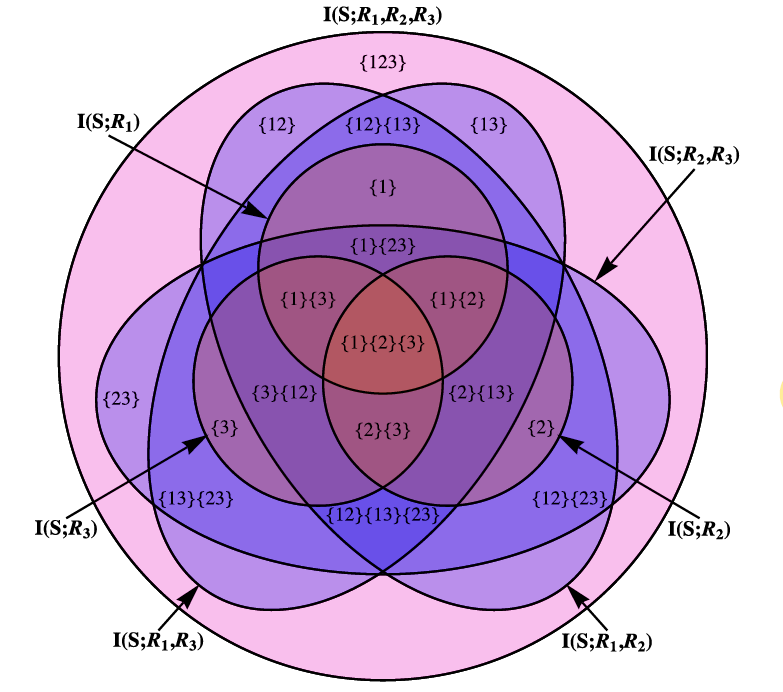
\includegraphics[width=0.8\linewidth]{img/partial4.png}
            \caption{PI diagram for 4 variables.}
            \label{fig:pi4}
        \end{figure}
    \end{column}
    \end{columns}
\end{frame}





\section{PI-Measure}

We next show how redundancy measure can be formulated in a set-theoretic way. In this chapter, we develop a theory which establishes a one-to-one correspondence between set theory and partial information measures, as well as their decomposed values, namely $I_{\min}$ and $\Pi_{\mathbf{R}}$. Unlike the scenario where relationship between entropies and mutual information is formed, the correspondence here involves more atomic sets and more complicated set properties.

\subsection{Formulation}

In this section, using the notion of measure theory introduced in Chapter 2, % todo!!,
we will give a formal definition for the correspondence. To fix ideas, we first formulate in this section the one-to-one correspondence between redundancy measures and set theory for a three dimensional random source vector.

\paragraph{Field Generation}
For random variables $A_1$, $A_2$ and $A_3$ in $\mathbf{A}$, let $\tilde{A_1}$, $\tilde{A_2}$ and $\tilde{A_3}$ be the sets corresponding to the information they provide to $S$ respectively, which is $I\left(S;A_i\right)$, or equivalently saying,  $I_{\min}\left(S;\left\{A_i\right\}\right)$. Note that the field generated by these three sets is not enough in representing the general picture. With a maximal field size of $2^n$, it fails to cover all possible combinations of information redundancy measures, since our partial information decomposition is based on the second-order power set of all sources.

As a result, a natural solution for our formulation is to take the first-order power set of sources as the atom field. In addition to $\tilde{A_1}$, $\tilde{A_2}$ and $\tilde{A_3}$, now we have to introduce $\tilde{A}_{12}$, $\tilde{A}_{23}$ , $\tilde{A}_{13}$ and $\tilde{A}_{123}$.

Formally, let $A_1,\ldots,A_{k^{'}}$ be nonempty and potentially dependent dimensions of sources $\mathbf{A}$. since the redundancy of a particular subset can be absorbed by its super-set, the field $\mathcal{F}$ is defined as any collections of sets which can be obtained by any sequence of usual set operations on \textit{basic sets} $\Gamma$, where 
\begin{equation}
    \Gamma = \left\{ \beta \in \mathcal{P}_{1}(\mathbf{A}) : \forall A_i,A_j \in \beta, {A}_i \nsubseteq {A}_j \right\}
\end{equation}

For every random variable collection in the $\Gamma$, its self-redundancy is defined as $I_{\min}\left(S;\left\{A_i, \ldots, A_j\right\}\right)$. We use $\left\{ \tilde{A}_{i}, \ldots, \tilde{A}_{j} \right\}$, or abbreviation $\tilde{A}_{i\ldots j}$ to represent the basic set its self redundancy corresponds to. Based on observations in Figure \ref{fig:pidiagram}, the set measure we've defined has the following correspondence with redundancy measure through operation of intersection.

\begin{equation}
    \mu^{*}\left(\tilde{A}_{i \ldots j} \cap \ldots \cap \tilde{A}_{m \ldots n} \right) = I_{\min}\left(S; \left\{{A}_i,\ldots,{A}_j \right\}, \ldots,  \left\{{A}_m,\ldots,{A}_n \right\}\right)
    \label{eqn:intersectofbasic}
\end{equation}

% State Lemmas about atom-intersection, atom-union, atom-complementary(omega=0)


% nonnegative of measure




\paragraph{Symbolic Substitution}
The equation above fails to cover other kinds of set operations like difference and union. In fact, due to the complexity of partial information, we can't write the direct PI correspondence of these operations.

Luckily, Chapter \ref{sec:partialdecompositon}  has provided us with a useful tool, partial information $\Pi_{\mathbf{R}}$. Recall that partial information is the basic, non-intersecting building block of any redundancy measures, including their arbitrary sums of differences. With partial information, we can formally write out the symbol correspondence between sets and redundancy measures. The substitution strategy is listed as follows.

\begin{enumerate}
    \item For every basic sets $\tilde{A}_{i\ldots j}$, $\mu^{*} \left(\tilde{A}_{i\ldots j}\right) = I_{\min}\left(S;\left\{A_i, \ldots, A_j\right\}\right)$.
    \item For any two sets $\alpha$in the field, $\mu^{*} \left(\alpha^{c} \right) = \sum_{ \alpha \prec \gamma  } \Pi_{\mathbf{R}} (S;\gamma)$
    \item For any two sets $\alpha$ and $\beta$ in the field, $\mu^{*} \left(\alpha \cap \beta \right) = \sum_{\gamma \preceq \alpha \text{ and } \gamma \preceq \beta} \Pi_{\mathbf{R}} (S;\gamma)$
    \item For any two sets $\alpha$ and $\beta$ in the field, $\mu^{*} \left(\alpha \cup \beta \right) = \sum_{\gamma \preceq \alpha \text{ or } \gamma \preceq \beta} \Pi_{\mathbf{R}} (S;\gamma)$
    \item For any two sets $\alpha$ and $\beta$ in the field, $\mu^{*} \left(\alpha - \beta \right) = \sum_{\gamma \preceq \alpha \text{ and } \beta \prec \gamma} \Pi_{\mathbf{R}} (S;\gamma)$
\end{enumerate}

By the definition of fields, every set in the diagram can be represented as a $\cap$ or $\cup$ combination of basic sets or its complement. With the strategy above, we have formally defined the \textit{PI-Measure} in terms of measure theory. 



\subsection{Simplification}

There are two problems with our definition. One is that the basic sets, sets that generate fields are growing too fast as the number of random variable increases. And the other is that the correspondence we've defined for arbitrary sets is too complex to be of practical use. In this section, we will try to eliminate redundant fields in order to address the first problem and find alternative, useful expressions of fields by means of set theory.

\paragraph{Eliminate Redundant Fields} An important usage of set-theory in information theory is to use Venn diagram to help derive formulas. Now, with the extra power-sets of sources as basic sets, it is impractical to plot redundancy information sets out as we did with Shannon information measures. However, the basic sets here are not independent with each other. For example, $I(S;R_1,R_2)$ clearly has no complement intersecting with $I(S;R_1)$ and $I(S;R_2)$. Hence, as what we did with Markov Chain in Chapter \ref{sec:markov}, we can also derive some useful formulas to eliminate non-existing fields, in order to simplify the diagram.\footnote{We should not confuse empty sets with sets that have a measure of zero. In other words, the reason why we don't plot these sets out is because their measures are zero, not that these sets don't `exist'.}

To fix ideas, we take the multivariate information of three variables $I(S;{A}_1, {A}_2)$ as example, note that $\left\{ \tilde{A}_1 \right\} \subseteq \left\{\tilde{A}_1, \tilde{A}_2 \right\}$. It follows that 
\begin{equation}
\begin{aligned}
    \mu^{*}\left( \left\{ \tilde{A}_1 \right\} \cap \left\{\tilde{A}_1, \tilde{A}_2 \right\}^{C} \right) &= \mu^{*}\left( \left\{\tilde{A}_1\right\}\right)  - \mu^{*}\left(\left\{\tilde{A}_1 \right\}\cap  \left\{  \tilde{A}_1, \tilde{A_2} \right \} \right) \\
    &= I_{\min} \left( S; \left\{\mathbf{A}_1 \right\} \right) - I_{\min} \left( S; \left\{ \mathbf{A}_1 \right\} ,\left\{ \mathbf{A}_1, \mathbf{A}_2 \right\} \right) = 0
\end{aligned}
\label{eqn:fieldelim}
\end{equation}

% Normal form in atom:
% [~]() nonintersected-union/minus of sets...


Similarly, with the observation that $\left\{ \tilde{A}_2 \right\} \subseteq \left\{\tilde{A}_1, \tilde{A}_2 \right\}$, we have $\mu^{*}\left( \left\{ \tilde{A}_2 \right\} \cap \left\{\tilde{A}_1, \tilde{A}_2 \right\}^{C} \right) = 0$. As has been proved in \ref{thm:nonneg} that all regions should have a non-negative measure, the sub-regions will also preserve a zero measure. Hence, three starred regions in Figure \ref{fig:elim3} will have a zero measure. To make our diagram more legible, we can erase these three regions out.


\begin{figure}
\centering
\subfigure[Before Elimination]{
\begin{minipage}[t]{0.5\linewidth}
\centering
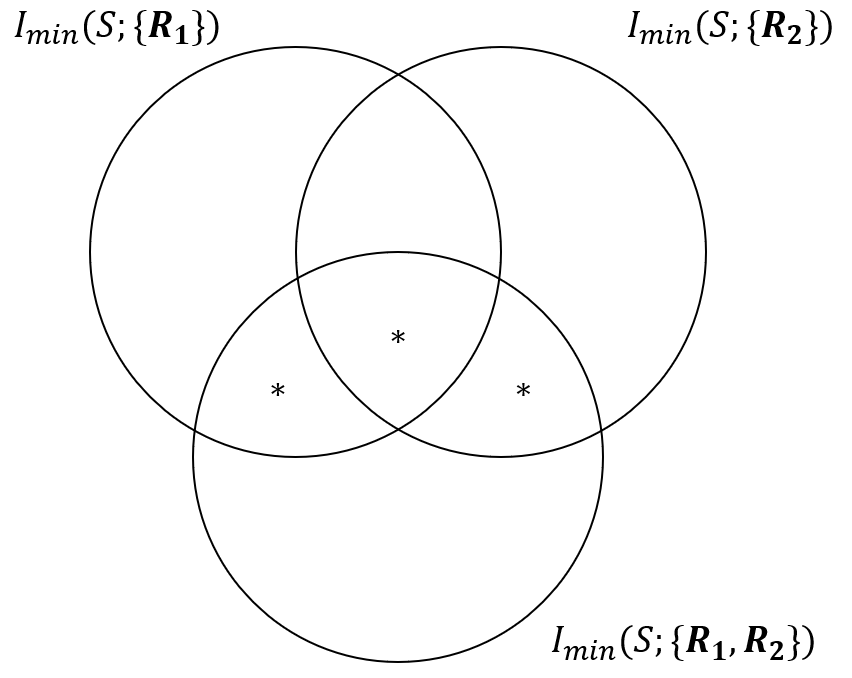
\includegraphics[height=4.5cm]{img/elim1.png}
%\caption{fig1}
\end{minipage}%
}%
\subfigure[After Elimination]{
\begin{minipage}[t]{0.5\linewidth}
\centering
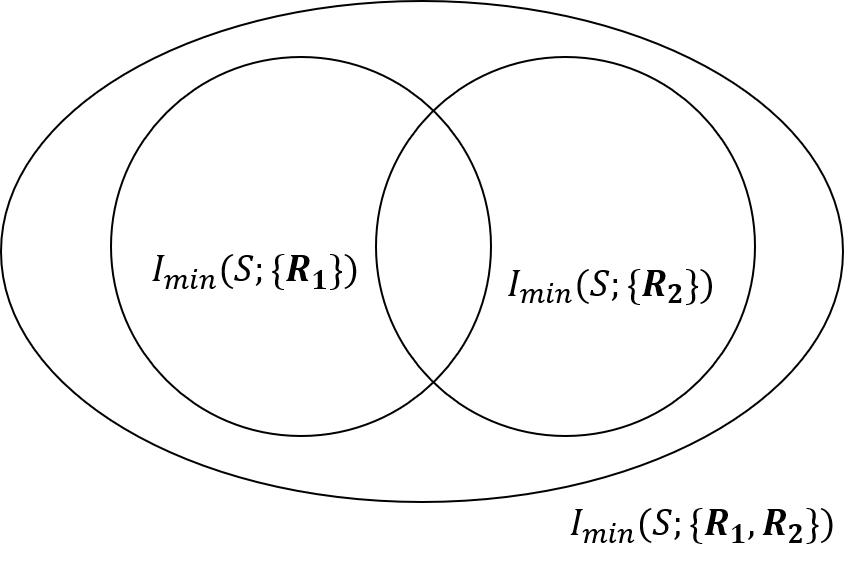
\includegraphics[height=4.5cm]{img/elim2.png}
%\caption{fig2}
\end{minipage}%
}%
\centering
\caption{Field Elimination for 2 Source Variables}
\label{fig:elim3}
\end{figure}

As the number of variables increases, the complexity of the combination also grows exponentially. It becomes nontrivial to identify all the subset relations, especially when higher-order fields are generated. Here is a formulated rule to follow.

\begin{theorem}[Field Elimination] For any two basic sets $\tilde{A}_{i\ldots j} , \tilde{A}_{i' \ldots j'} \in \Gamma$, if $\tilde{A}_{i\ldots j} \subseteq \tilde{A}_{i' \ldots j'}$, then the measure of any set intersection with $\tilde{A}_{i\ldots j} \cap \tilde{A}_{i' \ldots j'}^{C}$ is zero.
\begin{proof}
 The proof that $\mu^{*}\left( \left\{ \tilde{A}_{i\ldots j} \right\} \cap \left\{\tilde{A}_{i'\ldots j'} \right\}^{C} \right) = 0$ follows a similar pattern as Equation \ref{eqn:fieldelim}. For any set $\eta$ that intersects with $ \left\{ \tilde{A}_{i\ldots j} \right\} \cap \left\{\tilde{A}_{i'\ldots j'} \right\}^{C}$, by the non-negativity of partial information measure, we have
  \begin{equation}
     0 \le \mu^{*}\left(\eta  \cap \left\{ \tilde{A}_{i\ldots j} \right\} \cap \left\{\tilde{A}_{i'\ldots j'} \right\}^{C} \right) \le \mu^{*}\left( \left\{ \tilde{A}_{i\ldots j} \right\} \cap \left\{\tilde{A}_{i'\ldots j'} \right\}^{C} \right) = 0
\end{equation}
\end{proof}
\end{theorem}

The above theorem also implies a strategy to plot a pretty partial information diagram. Starting with singleton basic sets, every time we draw a new basic set, check the subset relation with the existing sets and eliminate the intersecting fields out. A construction of partial information diagram for four random variables is shown in Figure \ref{fig:elim4}. With such strategy, we can make clear how the partial information diagram in Figure \ref{fig:pidiagram} is step-by-step formulated with a set theoretic view.


\begin{figure}
\centering
\subfigure[$\tilde{A}_3$ produces no extra redundant fields]{
\begin{minipage}[t]{0.3\linewidth}
\centering
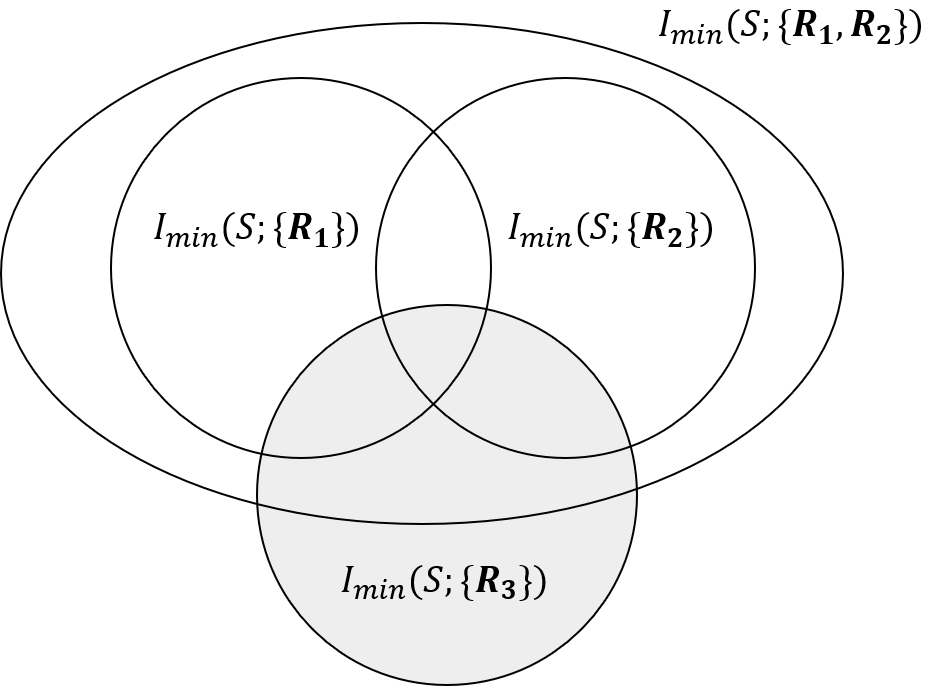
\includegraphics[height=3.5cm]{img/decompose1.png}
%\caption{fig1}
\end{minipage}%
}%
\quad
\subfigure[Adding Basic Set $\tilde{A}_{12}$ produces extra redundant fields as has been starred]{
\begin{minipage}[t]{0.3\linewidth}
\centering
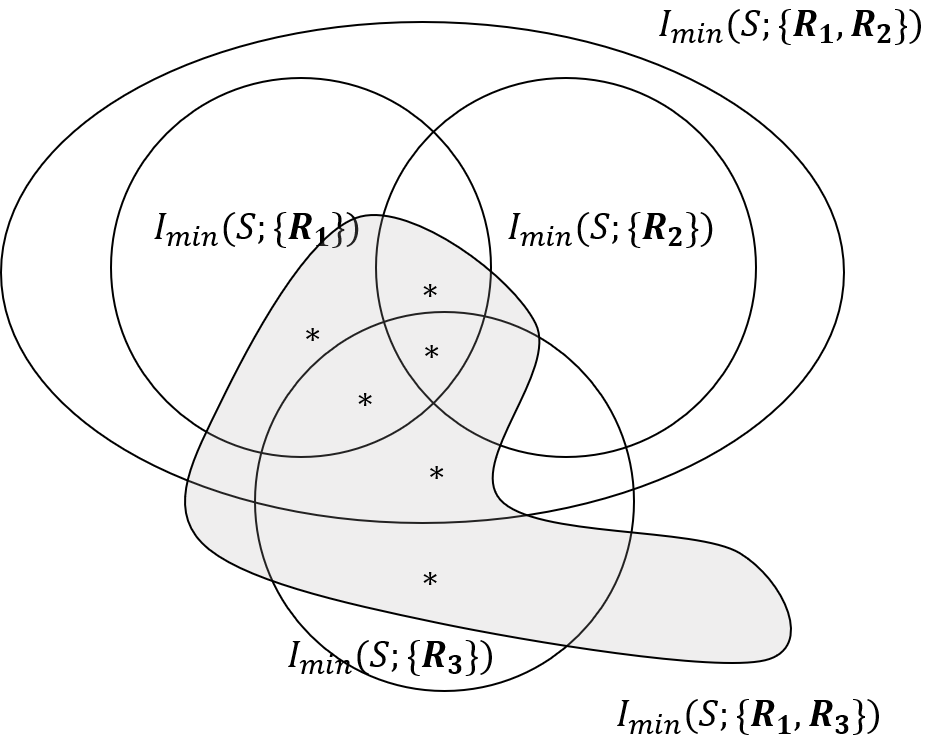
\includegraphics[height=3.5cm]{img/decompose2.png}
%\caption{fig2}
\end{minipage}%
}%
\quad
\subfigure[After Elimination]{
\begin{minipage}[t]{0.3\linewidth}
\centering
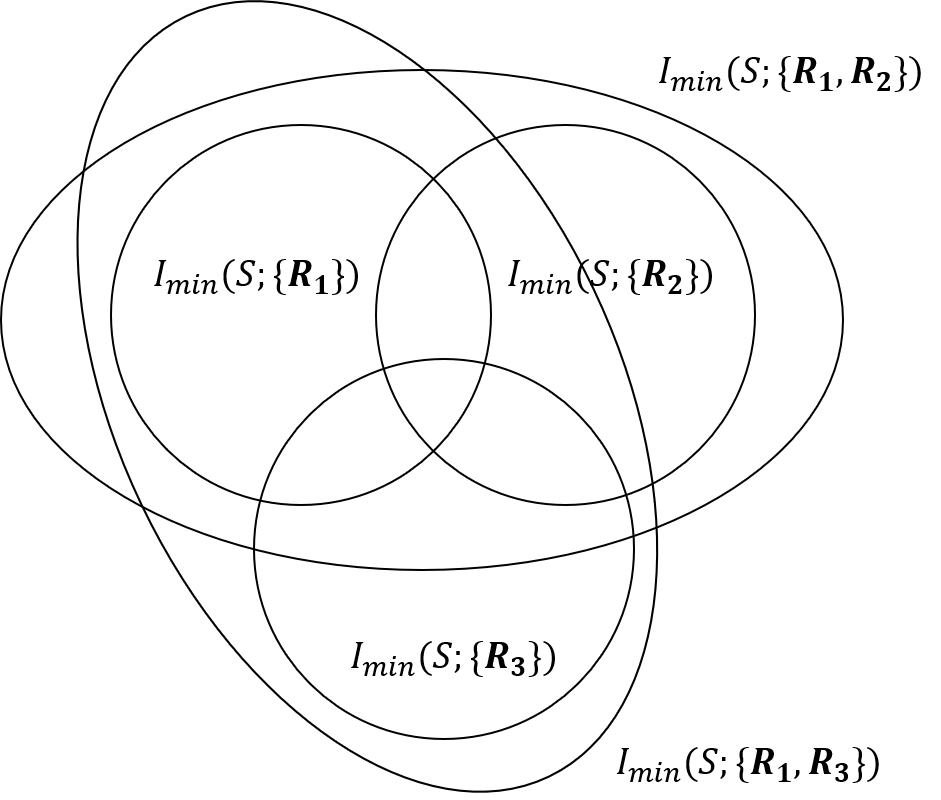
\includegraphics[height=3.5cm]{img/decompose3.png}
%\caption{fig2}
\end{minipage}%
}%
\centering
\caption{Field Elimination Strategy for 3 Source Variables}
\label{fig:elim4}
\end{figure}


\paragraph{Alternative Field Expressions} Note that the partial information $\Pi_{\mathbf{R}}$ is actually a derived concept. In common cases, we are more interested in the redundancy measure, which has more practical implications. We try to derive the relation between arbitrary field and linear combinations of redundancy measure from a pure set-theoretic view.

% Similar to Shannon information measure, we can define the \textit{universal set}
% \begin{equation}
%     \Omega = \bigcup_{i\in\mathcal{N}_n} \tilde{A}_i
% \end{equation} where the index set $\mathcal{N}_n$ is defined as

% \begin{equation}
%     \mathcal{N}_n = \mathcal{P}_1\left(\left\{ 1,2,\ldots,n\right\}\right)
% \end{equation}


Note that the measure of \textit{atoms} in $\mathcal{F}_n$ are a perfect matching to the partial information $\Pi_{\mathbf{R}}$. The reason is that by Definition \ref{def:partial}, $\Pi_\mathbf{R}\left(S;\alpha\right)$ only provides the unique information from $\alpha$. There is no possibility that the sets corresponding to a single partial information can be deposed to smaller sets by intersection, which coincides with the property of set atoms.

With the observation above, we can narrow our scope into atoms, since the measure of arbitrary set can be written into a combination of atoms. Because all atoms can be represented as sets of 

\begin{equation}
    \cap _{i\in\mathcal{N}_n} \tilde{Y}_i (\tilde{Y}_i = \tilde{A}_i \text{ or } \tilde{A}_i^c), \text{ where the index set } \mathcal{N}_n = \mathcal{P}_1\left(\left\{ 1,2,\ldots,n\right\}\right)
\end{equation}

we only need to study two operations, namely complement and intersection,  on basic sets $Y_{i \in \mathcal{N}_n}$. The mapping of such operations to redundancy measures can be listed as follows.

\begin{align}
    & \mu^{*}\left( \tilde{A}_{N_1} \cap \ldots \cap \tilde{A}_{N_k} \cap \tilde{A}_{M_1}^{C} \cap \ldots\cap \tilde{A}_{M_j}^{C} \right) \\
    &= \mu^{*}\left(\tilde{A}_{N_1} \cap \ldots \cap \tilde{A}_{N_k} \right) - \sum_{i=1}^{k} \mu^{*} \left( \tilde{A}_{N_1} \cap \ldots \cap \tilde{A}_{N_k} \cap\tilde{A}_{M_1} \cap \ldots \cap \tilde{A}_{M_i} \right) \label{eqn:simplify} \\  
    & \text{where } \left\{ N_1, \ldots, N_k, M_1, \ldots, M_k \right\} = \mathcal{N}_n \label{eqn:idxsetatom}
\end{align}

The formula above is not hard to obtain from a pure set-theoretic perspective, now note that in Equation \ref{eqn:simplify}, all the sets being measured are intersections of basic sets. By applying Equation \ref{eqn:intersectofbasic}, we can write them out in the form of redundancy measure $I_{\min}$. By now, we have finished proving that any atom can be written as a $\pm 1$ combination of some redundancy measures.

Therefore, we can conclude that any field can be written as
a linear combination of redundancy measures. An application of such expression is to calculate partial information in a top-down way. In the next chapter we will apply such strategy to show how our method can eliminate the need to calculate lots of partial information in the traditional bottom-up strategy.

Note that if we change the equality into $\subseteq$ in Equation \ref{eqn:idxsetatom}, the formula will still hold, i.e. we can always write out the intersection of any basic sets or their complements in the form of Equation \ref{eqn:simplify}, which may help us reduce the complexity of computing redundancy a step further.

\subsection{Completeness}
In order to validate the effectiveness of the PI-measure correspondence, we will close our formulation section with a conclusion that the measure of any field can be completely obtained from the measures of basic sets.


\begin{theorem}
Let
\begin{equation}
    \mathcal{B} = \left\{ \tilde{X}_{G}: G \text{ is a nonempty subset of  }\mathcal{N}_n \right\}
\end{equation}
Then a measure $\mu^{*}$ on $\mathcal{F}_n$ is completely specified by $\left\{ \mu^{*}(B), B \in \mathcal{B} \right\}$, which can be any set of real numbers.

\begin{proof}
The number of elements in $\mathcal{B}$ is equal to the number of nonempty subsets of $\mathcal{N}_{n},$ which is $2^{2^{n}-1}-1 .$ Thus $|\mathcal{A}|=|\mathcal{B}|=2^{2^{n}-1}-1  .$ Let $k=2^{2^{n}-1}-1 $ Let $\mathbf{u}$ be a column $k$ -vector of $\mu(A), A \in \mathcal{A},$ and $\mathbf{h}$ be a column $k$ -vector of $\mu(B), B \in \mathcal{B} .$ since all the sets in $\mathcal{B}$ can expressed uniquely as the union of some nonempty atoms in $\mathcal{A},$ by the set-additivity of $\mu,$ for each $B \in \mathcal{B}, \mu(B)$ can be expressed uniquely as the sum of some components of u. Thus
\begin{equation}
\mathbf{h}=C_{n} \mathbf{u}
\label{eqn:completeness1}
\end{equation}
where $C_{n}$ is a unique $k \times k$ matrix. On the other hand, it has been shown that for each $A \in \mathcal{A}, \mu^{*}(A)$ can be expressed as a linear combination of $\mu(B), B \in \mathcal{B}$ by applications, if necessary, of Equation \ref{eqn:simplify}.

However, the existence of the said expression does not imply its uniqueness. Nevertheless, we can write
\begin{equation}
\mathbf{u}=D_{n} \mathbf{h}
\label{eqn:completeness2}
\end{equation}
for some $k \times k$ matrix $D_{n} .$ Upon substituting Equation \ref{eqn:completeness1} into Equation \ref{eqn:completeness2}, we obtain
\begin{equation}
\mathbf{u}=\left(D_{n} C_{n}\right) \mathbf{u}
\label{eqn:completeness3}
\end{equation}
which implies that $D_{n}$ is the inverse of $C_{n}$ as Equation \ref{eqn:completeness3} holds regardless of the choice of $\mu .$ since $C_{n}$ is unique, so is $D_{n} .$ Therefore, $\mu^{*}(A), A \in \mathcal{A}$ are uniquely determined once $\mu^{*}(B), B \in \mathcal{B}$ are specified. Hence, a measure $\mu^{*}$ on $\mathcal{F}_{n}$ is completely specified by $\{\mu(B), B \in \mathcal{B}\},$ which can be any set of real numbers. The theorem is proved.

\end{proof}

\end{theorem}

\section*{Summary}

\begin{frame}{Summary}
  \begin{block}{Previous Work}
    \begin{itemize}
    \item Correspondence between Shannon information and set theory
    \item Redundancy measure and partial information decomposition methods for multivariate information
    \end{itemize}
  \end{block}


  \begin{block}{Achieved Goals}
    \begin{itemize}
    \item Formalize the correspondence between redundancy measure and set theory
    \item Prove the completeness of the correspondence relation
    \item Simplify the correspondence expressions
    \item Propose a top-down strategy to calculate redundancy measure
    \end{itemize}
  \end{block}
\end{frame}

% Bibliography section. Use \bibitem to add more bibliography items.
\section*{Bibliography}
\begin{frame}{Bibliography}
  \begin{thebibliography}{10}

  \bibitem{nonneg}
    Paul L. Williams, Randall D. Beer.
    \newblock {Nonnegative Decomposition of Multivariate Information[J]}
    \newblock arXiv preprint arXiv:1004.2515, 2010.
  \bibitem{book}
    Yeung R W.
    \newblock {Information theory and network coding[M]}
    \newblock Springer Science \& Business Media, 2008.
  \end{thebibliography}
\end{frame}


% \begin{frame}

% \begin{center}
% \begin{Large}
% The End

% \vspace{10pt}

% Thanks!
% \end{Large}
% \end{center}

% \end{frame}

\end{document}
